\chapter{Mécanique des fluides}
\section{Fluide au repos}
\subsection{Loi fondamentale de la statique des fluides}

Pour un fluide au incompressible (\(\rho = \text{cste}\)), au repos dans un réferentiel galiléen et placé dans un champ de pensenteur uniforme, la pression ne dépend que de \(z\). On a : 
\[
    P(z) = P_{0}+\rho gz
\]
Avec :
\begin{itemize}
    \item \(P(z)\) la pression à \(z\)
    \item \(P_{0}\) la pression à \(z=0\) 
    \item \(\rho \) en \(\text{kg} \cdot \text{m}^{-3}\)
    \item \(g\) l'intensité du champ de pesanteur.   
\end{itemize}

\begin{remark}[sens de l'axe]\label{}
    Si l'axe vertical \((Oz)\) est orienté vers le bas, alors on a \(P(z)-P_{0} \propto z\)  
\end{remark}

\section{Poussée d'Archimède}
\subsection{Cas d'un cylindre vertical}

\begin{figure}[!htb]
    \centering
    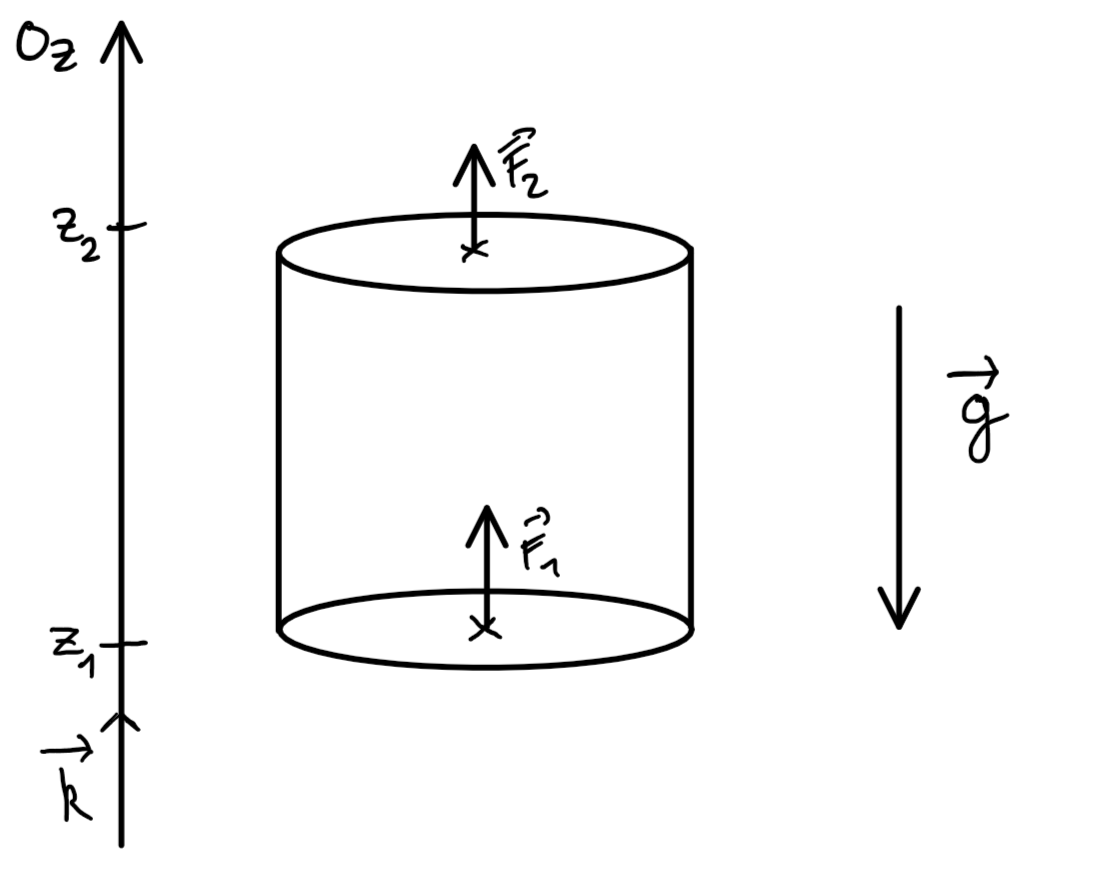
\includegraphics[width=0.8\textwidth]{SchemaPA.png}
    \caption{Schema de la poussée d'archimède sur un cylindre}
    \label{fig:SchemaPA}
\end{figure}

On considère un cylindre vertical de section \(S\) et d'hauteur \(h\) plongé dans un fluide incompressible de masse volumique \(\rho \). On effectue le bilan des forces pressantes appliquées aux cylindres. \\
Cette force se décompose en trois composantes : 
\begin{itemize}
    \item Sur la face latérale, les forces pressantes s'annulent, on a : \(\sum \vec{F} = \vec{0}\)
    \item A l'altitude \(z = z_{1}\), \(\vec{F}_{1} = P(z_{1})S \cdot \vec{k} = (P_{0}+\rho g z_{1})S \cdot \vec{k}\)   
    \item A l'altitude \(z = z_{2}\), \(\vec{F}_{2} = -P(z_{2})S \cdot \vec{k} = -(P_{0}+\rho g z_{2})S \cdot \vec{k}\)
\end{itemize}
D'après la loi de la statique des fluides, on a : \\
\begin{eqnarray*}
    P_{1}-P_{2} &= P_{0} -\rho g z_{1} - (P_{0} - \rho g z_{2})\\
    &= \rho g(z_{2}-z_{1}) (\text{axe vers le haut})
\end{eqnarray*}

On a donc : \(\sum \vec{F} = \vec{F}_{1} + \vec{F}_{2} = \rho g (z_{2} - z_{1})S \vec{k}\) D'ou : \\
\[
    \sum \vec{F} = -\rho V \vec{g} \, \square
\] 

Le cylindre est donc soumis à une force pressante exercée par le fluide qui l'entoure égale à l'opposée du poids du fluide déplacé. Cette force pressante est appelée la poussée d'Archimède. 

\subsection{Généralisation}

\begin{theorem}[Généralisation]\label{thm:}
    La résultat précédent peut être généralisé à tout corps plongé dans un fluide : c'est la poussée d'Archimède : \\
    "Tout corps plongé dans un fluide au repos subit une force dont a valeur est égale au poids du fluide déplacé."   
    \[
        \vec{\Pi} _{A} = -\rho V \vec{g}
    \]
\end{theorem}


